\section{Anexo A: Calibración del campo magnético}
\label{anexo:a}

Al comenzar la calibración, se comenzó con el valor de resistencias dadas por Pandiani y Sarasola \cite{Pandiani}. A partir
de dichos valores se midió el campo magnético a lo largo del cilindro. Las zonas con un bajo $|\mathbf{B}|$ indicaban que se necesitaba más corriente
por lo que se disminuían las resistencias de los reóstatos de las bobinas de dicha zona. De manera análoga, si el campo magnético era demasiado alto, se aumentaban las resistencias.
Este proceso se repitió reiteradas veces hasta alcanzar un campo lo suficientemente homogéneo. Esto se alcanzó para los valores de resistencia presentados en la Tabla \ref{tab:resistencias}.

\begin{table}[h]
    \centering
    \begin{tabular}{cS}
        \toprule
        Reóstato & {Resistencia (\unit{\ohm})} \\
        \hline
        A1 & 32,3 \pm 0,1 \\
        A2 & 60,0 \pm 0,1\\
        A3 & 22,4 \pm 0,1 \\
        B1 & 3,1 \pm 0,1 \\
        B2 & 4,5 \pm 0,1 \\
        \bottomrule
    \end{tabular}
    \caption{Resistencias finales de los reóstatos para cada bobina.}
    \label{tab:resistencias}
\end{table}

Se hicieron barridos para distintos valores de corriente y se midió el campo magnético en distintos puntos del cilindro.
Con los datos se cada corriente, se tomó un valor promedio de $B$ a lo largo del cilindro y se ajustó dicho valor en función de la corriente. El resultado se muestra en la Figura \ref{fig:calibracion}.

\begin{figure}[!h]
    \centering
    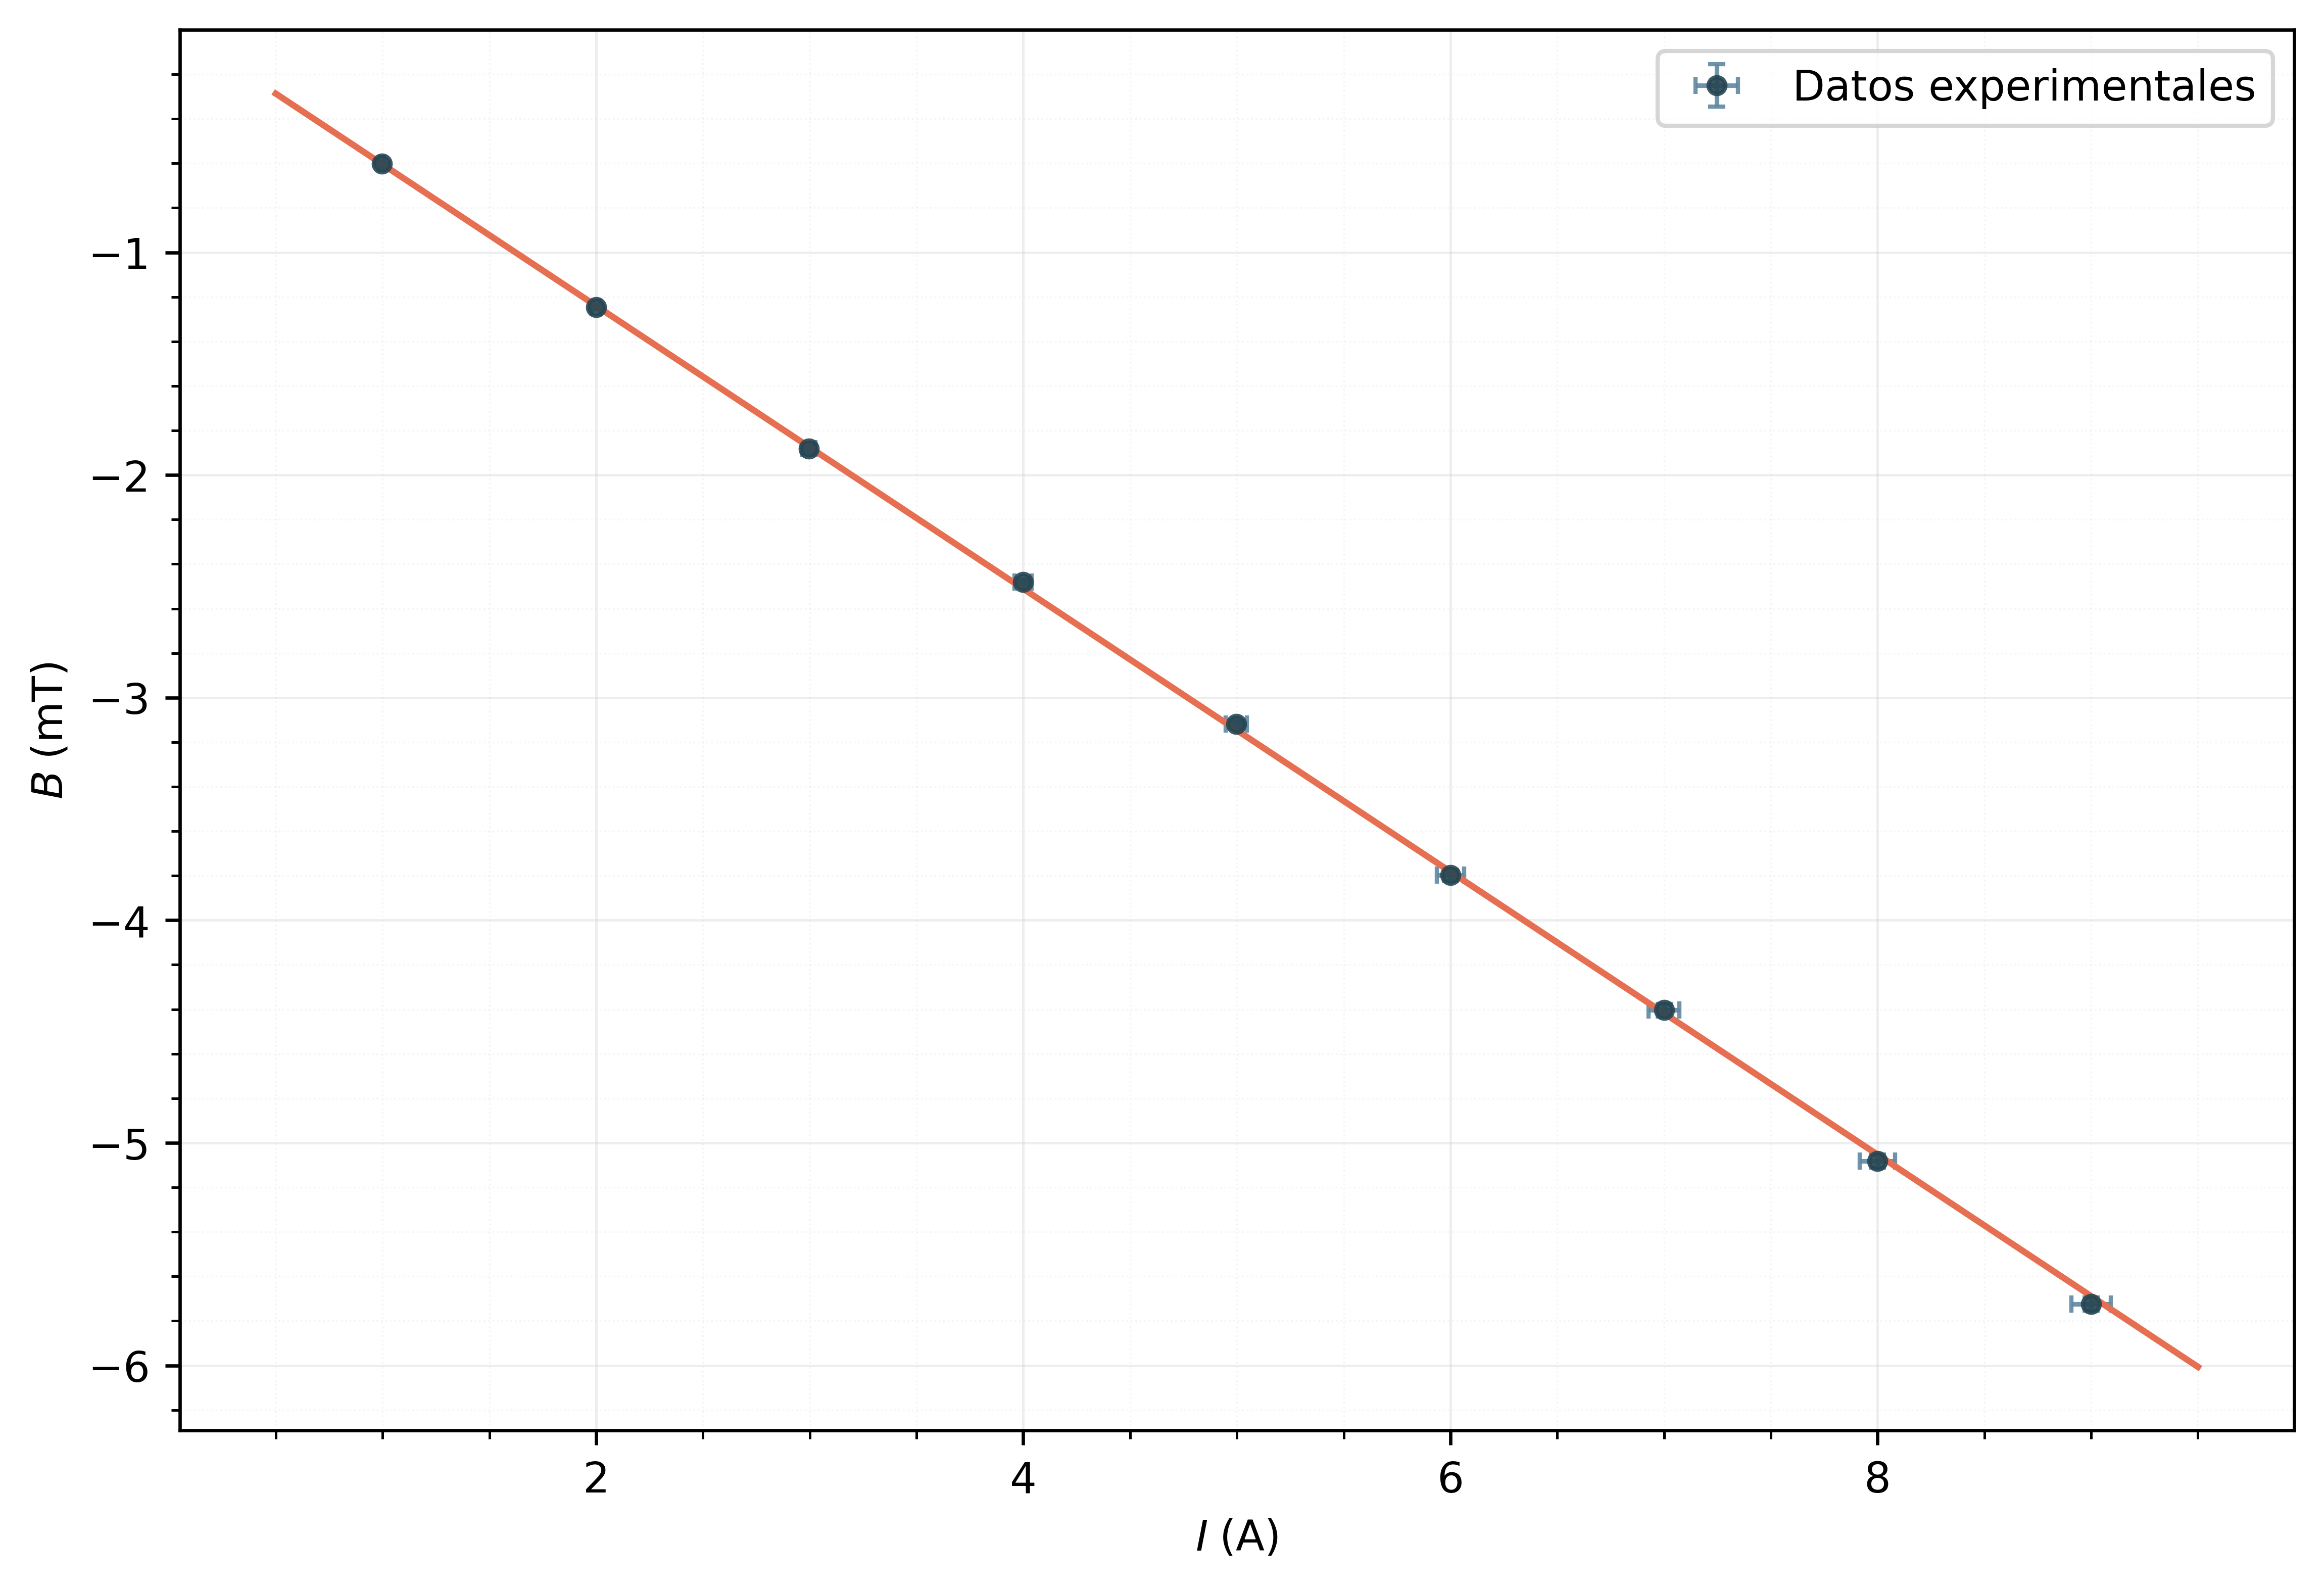
\includegraphics[width=0.45\textwidth]{Images/ajusteBI.png}
    \caption{Curva de calibración del campo magnético en función de la corriente.}
    \label{fig:calibracion}
\end{figure}

\section{Anexo B: Calibración de la fuente de corriente e identificación de mínimos}
\label{anexo:b}

Debido a que la fuente usada inicialmente para alimentar las bobinas, la GW Instek PSH-3620A, no entregaba la corriente que 
decía entregar, se optó por el uso de una fuente HP 6268B, la cual se comandaba analógicamente mediante una GW Instek GPS-4303S,
ya que esta necesita ser suministrada con tensión para entregar una corriente proporcional. Por esto se hizo una calibración de la fuente HP 6268B, para saber así que
corriente circula por el sistema en función de la tensión suministrada por la GPS-4303S. La curva de ajuste se muestra en la Figura \ref{fig: ajuste_fuente}

\begin{figure}[!h]
    \centering
    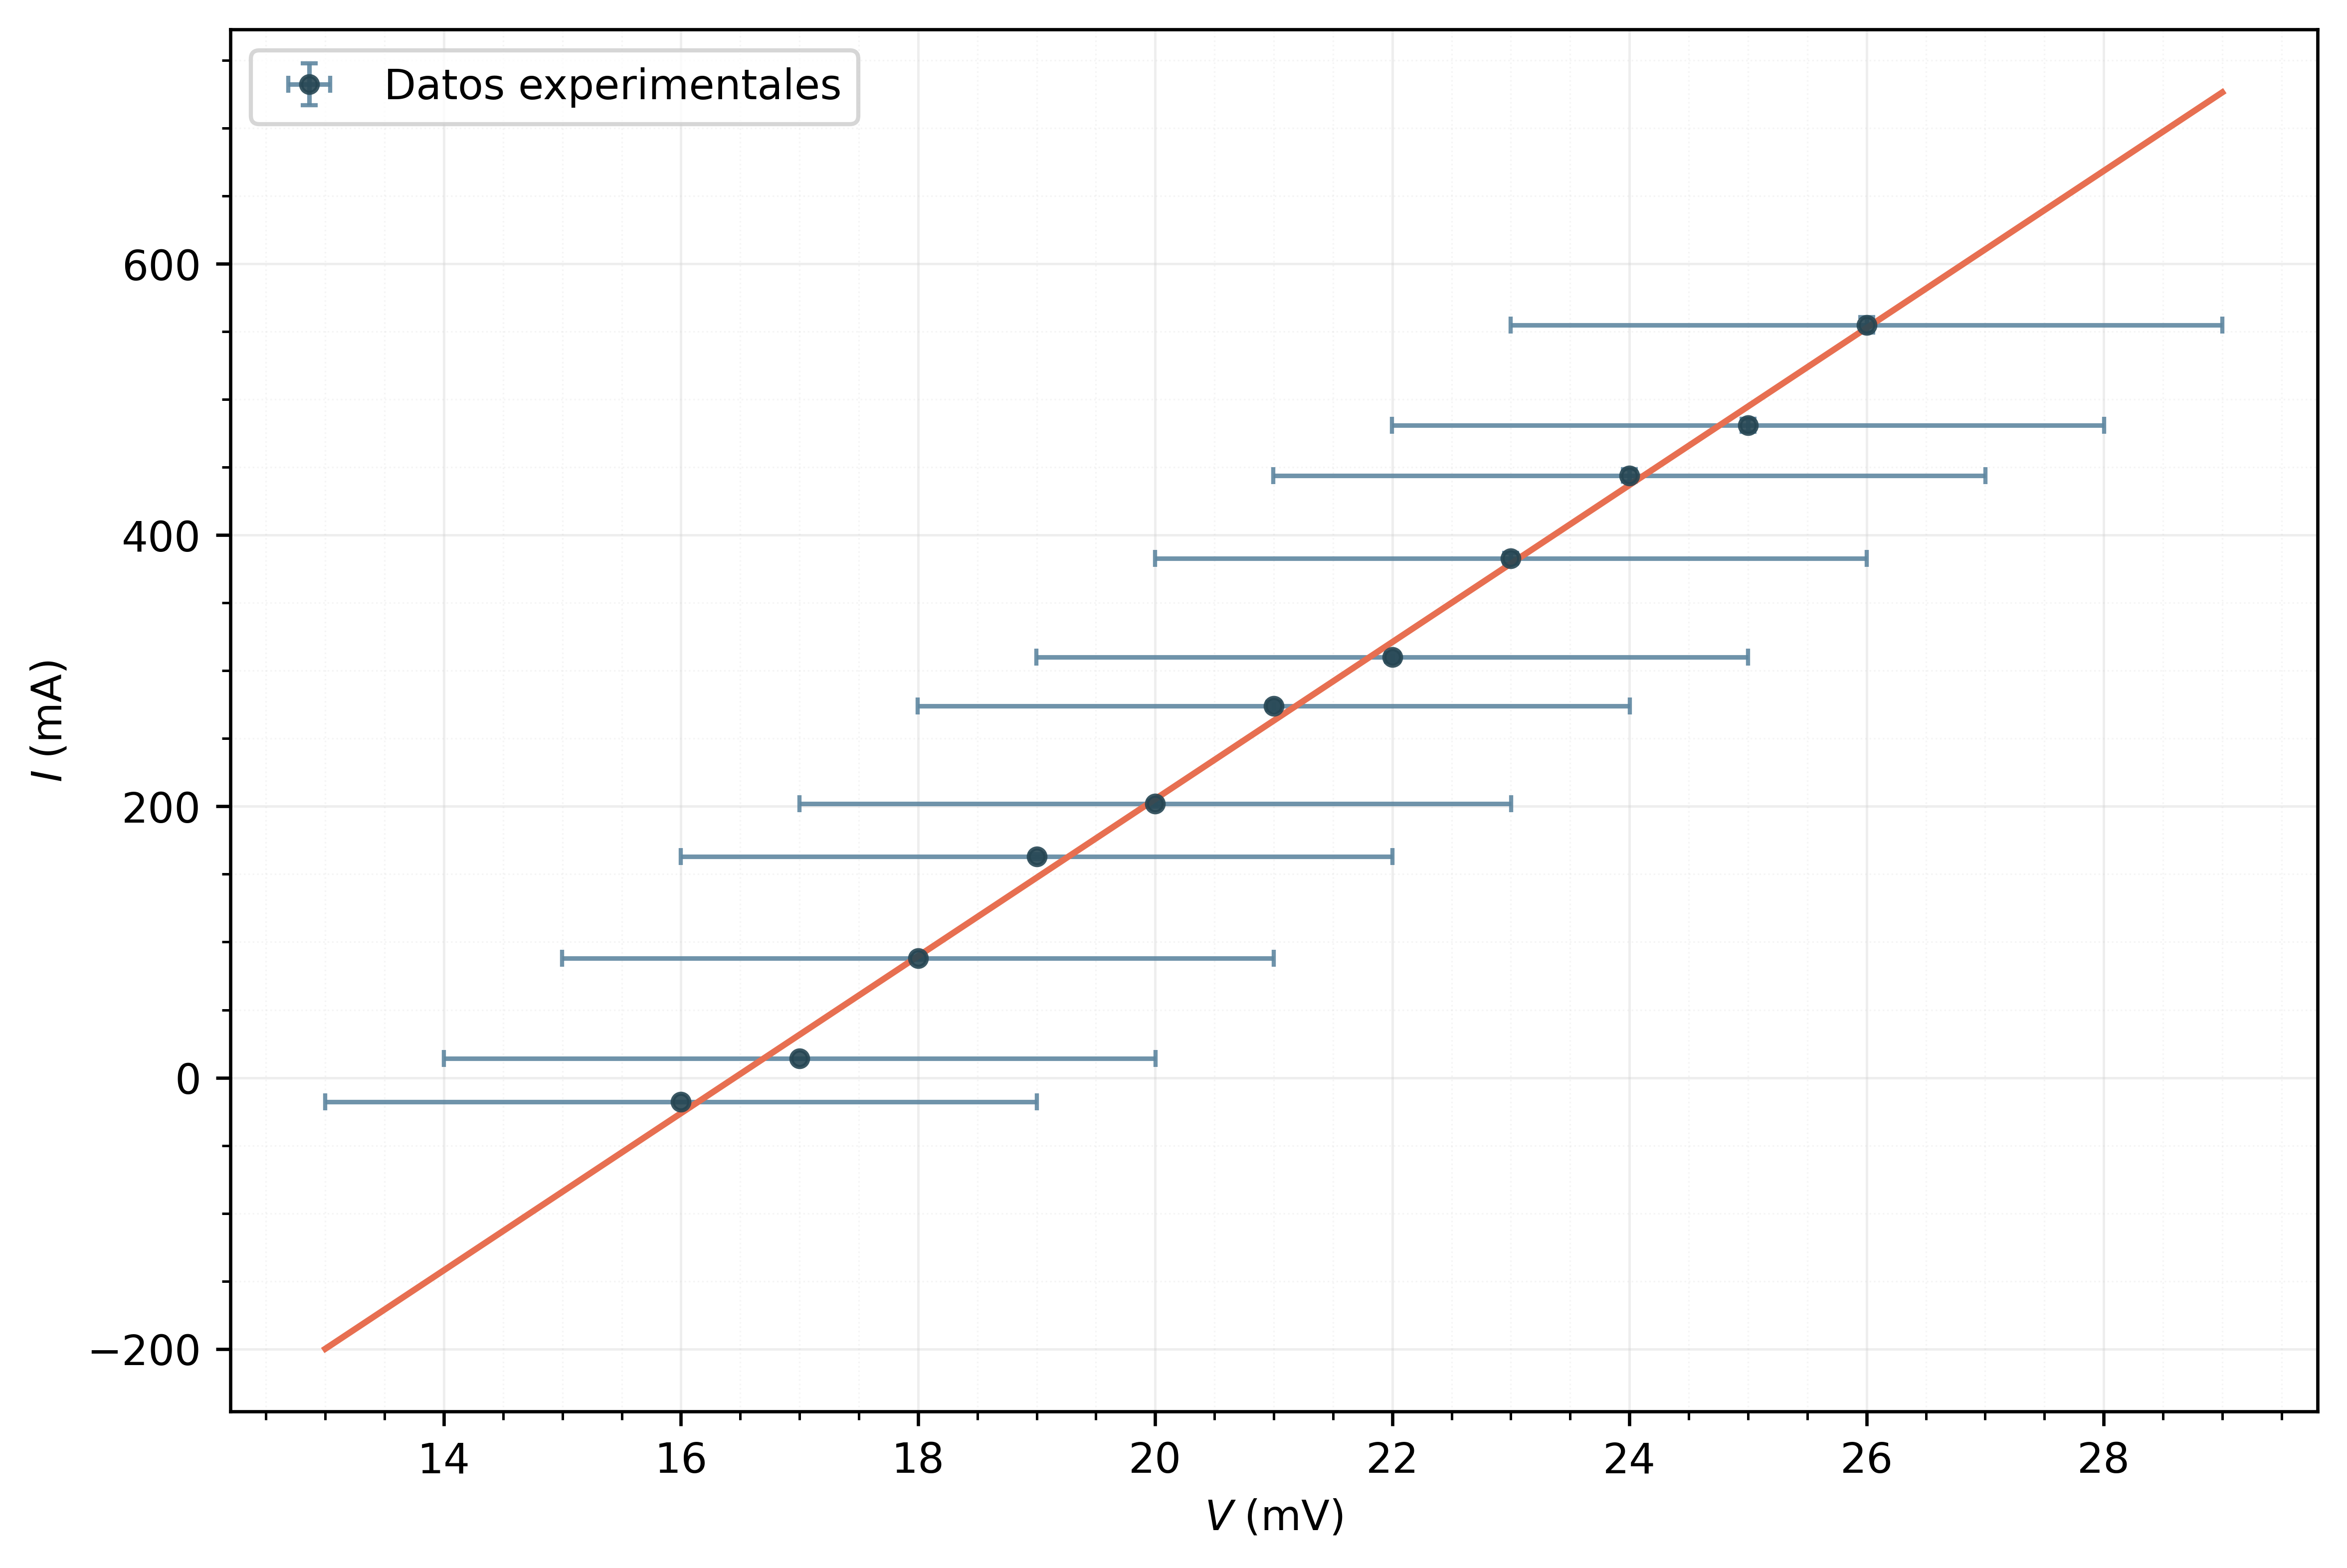
\includegraphics[width=0.49\textwidth]{Images/AjusteVI.png}
    \caption{Curva de calibración de la corriente entregada por la fuente HP 6268B en función de la tensión suministrada por la fuente GW Instek GPS-4303S.}
    \label{fig: ajuste_fuente}
\end{figure}

Luego para detectar los mínimos se hizo uso de un script de Python para comandar la cámara, tomar imágenes de la zona de impacto de los electrones,
calcular el área de impacto relativa, aumentar en $\SI{1}{\milli\volt}$ la tensión suministrada por la GPS-4303S, y repetir el proceso, almacenando los valores de tensión, área relativa y tensión de aceleración
utilizada en dicho barrido.

Para el cálculo del área de impacto relativa se toman los píxeles registrados y su intensidad. Si dicha intensidad es mayor a un umbral dado, llamado \textit{threshold}, se considerá que en ese píxel impactaron electrones.
Luego se calcula el área de impacto relativa como el número de píxeles que superan dicho umbral dividido por el número total de píxeles. Esto se hace para varios frames, a modo de tener un valor promedio de área relativa para cada tensión suministrada por la GPS-4303S.
